\documentclass[11pt,a4paper]{book}

% figure placement
% <https://stackoverflow.com/a/33801326>
\usepackage{float}
\let\origfigure\figure
\let\endorigfigure\endfigure
\renewenvironment{figure}[1][2] {
    \expandafter\origfigure\expandafter[H]
} {
    \endorigfigure
}

% fix for pandoc 1.14
\providecommand{\tightlist}{%
  \setlength{\itemsep}{0pt}\setlength{\parskip}{0pt}}

% TP: hack to truncate list of figures/tables.
\usepackage{truncate}
\usepackage{caption}
\usepackage{tocloft}
% TP: end hack

\usepackage{listings}
\usepackage{color}
\usepackage{geometry}
\usepackage{csquotes}
\usepackage{polyglossia}
\setmainlanguage{english}

\usepackage{setspace}
\usepackage{amssymb,amsmath}
\usepackage{ifxetex,ifluatex}
\usepackage{fixltx2e} % provides \textsubscript
\usepackage[utf8]{inputenc}

\usepackage{fontspec}
\usepackage{xltxtra,xunicode}
\usepackage{eurosym}

% typography
\setmainfont{SuisseWorks}
\setsansfont{SuisseIntl-Regular}
\setmonofont{IBMPlexMono}

\usepackage[
  final,
  protrusion=true,
  factor=1100,
  stretch=20
]{microtype}
\UseMicrotypeSet[protrusion]{basicmath} % disable protrusion for tt fonts

% <https://tex.stackexchange.com/a/404395>
\DeclareRobustCommand{\sbseries}{\fontseries{sb}\selectfont}
\DeclareTextFontCommand{\textsb}{\sbseries}

% footnotes
% <https://tex.stackexchange.com/a/54706>
\usepackage[hang,multiple]{footmisc}
\setlength{\footnotemargin}{1.5mm}
% <https://tex.stackexchange.com/a/141938>
\addtolength{\footnotesep}{1mm}

% charts
\usepackage{pgfplots}

\DeclareTextCommandDefault{\nobreakspace}{\leavevmode\nobreak\ } 

\defaultfontfeatures{Mapping=tex-text,Scale=MatchLowercase}

% use upquote if available, for straight quotes in verbatim environments
\IfFileExists{upquote.sty}{\usepackage{upquote}}{}
$if(geometry)$
  \usepackage[$for(geometry)$$geometry$$sep$,$endfor$]{geometry}
$endif$

$if(highlighting-macros)$
  $highlighting-macros$
$endif$

$if(tables)$
  \usepackage{longtable,booktabs}
$endif$

\usepackage{graphicx}

% git hash
\usepackage{xstring}
\usepackage{catchfile}
\CatchFileDef{\HEAD}{.git/refs/heads/master}{}
\newcommand{\gitrevision}{%
  \StrLeft{\HEAD}{7}%
}

$for(header-includes)$
$header-includes$
$endfor$

\makeatletter
\def\maxwidth{\ifdim\Gin@nat@width>\linewidth\linewidth\else\Gin@nat@width\fi}
\def\maxheight{\ifdim\Gin@nat@height>\textheight\textheight\else\Gin@nat@height\fi}
\makeatother

% Scale images if necessary, so that they will not overflow the page
% margins by default, and it is still possible to overwrite the defaults
% using explicit options in \includegraphics[width, height, ...]{}
\setkeys{Gin}{width=\maxwidth,height=\maxheight,keepaspectratio}

\usepackage[
  setpagesize=false,
  unicode=false,
  breaklinks=false,
  pdfusetitle,
  xetex
]{hyperref}
\usepackage{url}
\urlstyle{rm}

\hypersetup{
  bookmarks=true,
  colorlinks=true,
  linkcolor=teal,
  filecolor=gray,
  urlcolor=gray,
  citecolor=cyan,
  pdfborder={0 0 0},
}

$if(links-as-notes)$
  % Make links footnotes instead of hotlinks:
  \renewcommand{\href}[2]{#2\footnote{\url{#1}}}
$endif$

$if(strikeout)$
  \usepackage[normalem]{ulem}
  % avoid problems with \sout in headers with hyperref:
  \pdfstringdefDisableCommands{\renewcommand{\sout}{}}
$endif$

\setlength{\parindent}{0pt}
\setlength{\parskip}{6pt plus 2pt minus 1pt}
\setlength{\emergencystretch}{3em}  % prevent overfull lines

$if(numbersections)$
  \setcounter{secnumdepth}{5}
$else$
  \setcounter{secnumdepth}{0}
$endif$

\date{$date$}

% Table of contents formatting
\renewcommand{\contentsname}{Table of Contents}
\setcounter{tocdepth}{3}

% Headers and page numbering
\usepackage{fancyhdr}
\pagestyle{plain}

\usepackage{wallpaper}
\usepackage{ctable}

% Deal with 'LaTeX Error: Too many unprocessed floats.'
\usepackage{morefloats}
% or use \extrafloats{100}
% add some \clearpage

% % Chapter header
% \usepackage{titlesec, blindtext, color}
% \definecolor{gray75}{gray}{0.75}
% \newcommand{\hsp}{\hspace{20pt}}
% \titleformat{\chapter}[hang]{\Huge\bfseries}{\thechapter\hsp\textcolor{gray75}{|}\hsp}{0pt}{\Huge\bfseries}

\defaultfontfeatures{Mapping=tex-text} % converts LaTeX specials (``quotes'' --- dashes etc.) to unicode

%Attempt to set math size
%First size must match the text size in the document or command will not work
%\DeclareMathSizes{display size}{text size}{script size}{scriptscript size}.
\DeclareMathSizes{12}{13}{7}{7}

\usepackage{sectsty}
\usepackage[normalem]{ulem}

\sectionfont{\rmfamily\mdseries\Large}
\subsectionfont{\rmfamily\mdseries\scshape\large}
\subsubsectionfont{\rmfamily\mdseries\normalsize}

% captions
\usepackage[font={small,sf}]{caption}

% Adjust spacing between lines to 1.5
% \usepackage{setspace}
\setstretch{1.25}

\raggedbottom

% \usepackage[top=1.5in,bottom=1.5in,left=1.5in,right=1.4in]{geometry}
% \setlength\parindent{0.4in} % indent at start of paragraphs (set to 0.3?)
\setlength{\parskip}{9pt}

% Add space between pararaphs
% http://texblog.org/2012/11/07/correctly-typesetting-paragraphs-in-latex/
% \usepackage{parskip}
% \setlength{\parskip}{\baselineskip}

% references
\usepackage[authordate,doi=only,backend=biber]{biblatex-chicago}
$for(bibliography)$
\addbibresource{$bibliography$}
$endfor$

% tables
\usepackage{booktabs}
\usepackage{threeparttable}
\usepackage{array}
\newcolumntype{x}[1]{%
>{\centering\arraybackslash}m{#1}}%

% Allow for long captions and float captions on opposite page of figures
% \usepackage[rightFloats, CaptionBefore]{fltpage}

% Don't let floats cross subsections
% \usepackage[section,subsection]{extraplaceins}

% <https://github.com/rstudio/rmarkdown/issues/1649#issue-495777672>
\newlength{\cslhangindent}
\setlength{\cslhangindent}{1.5em}
\newenvironment{cslreferences}%
  %{$if(csl-hanging-indent)$\setlength{\parindent}{0pt}%
  %\everypar{\setlength{\hangindent}{\cslhangindent}}\ignorespaces$endif$}%
  {\par}

\begin{document}

\author{$for(author)$$author$$sep$ \and $endfor$}
\title{$title$}

% title page
\makeatletter
\newgeometry{margin=1in}
\begin{titlepage}
  \begin{center}
    \vspace*{2.5cm}
    
    {\huge\@title\unskip\strut\par}
    
    \vspace{8mm}
    
    \textit{by} \\ \vspace{2mm}
    {\Large \@author}

    % \vspace{12mm}

    \vspace{6mm}
    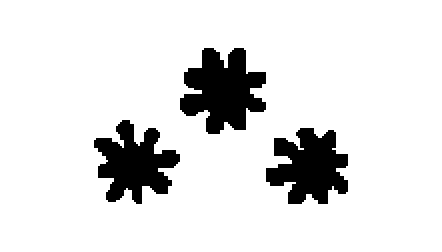
\includegraphics[width=0.075\textwidth]{layout/asterism-ulysses.png}
    \vspace{3mm}

    A thesis presented for the degree of \\ \vspace{2mm}
    {\Large Master of Science}
    
    \vfill

    \textit{at the} \\ \vspace{1mm}
    Institute of Computer Science \\
    Leipzig University, Germany \\ \vspace{3mm}

    \today\,— \texttt{\gitrevision} \\

    \vspace{3mm}
    
\includegraphics[width=0.5\textwidth]{layout/leipzig-university.eps}
    \vspace{8mm}

    % advisors  
    \begin{tabular}{cc}
      \begin{minipage}[c]{0.45\textwidth}
        \centering
        \textsb{Primary Advisor} \\
        Dr. Thomas Köntges \\
        Chair of Digital Humanities \\
        Leipzig University
      \end{minipage}

      \begin{minipage}[c]{0.45\textwidth}
        \centering
        \textsb{Secondary Advisor} \\
        Prof. Gregory Crane \\
        Department of Classical Studies \\
        Tufts University
      \end{minipage}
    \end{tabular}

  \end{center}
\end{titlepage}
\restoregeometry
\makeatother

\pagenumbering{gobble}

% license
Except where otherwise noted, content in this thesis is licensed under a Creative Commons Attribution-NonCommercial-NoDerivs 4.0 License (\url{https://creativecommons.org/licenses/by-nc-nd/4.0/}), which permits unrestricted use and distribution in any medium, provided the original work is properly cited and the material is not used for commercial purposes.

\vspace{2mm}

\includegraphics[width=0.25\textwidth]{layout/cc-nc-nd.pdf} \\

The source code of all Hyperwell repositories is available as open-source software and is licensed under a more permissive MIT License. \\

Copyright 2020, Jan Kaßel.


\pagebreak

% table of contents
\pagenumbering{gobble}
\tableofcontents
\newpage

$for(include-before)$
  $include-before$
$endfor$

$body$

$for(include-after)$
  $include-after$
$endfor$


\end{document}
